\documentclass[11pt]{article}
\usepackage[margin=1in]{geometry}
\usepackage{amsmath,amssymb,amsthm}
\usepackage{graphicx}
\usepackage{booktabs}
\usepackage{algorithm}
\usepackage[noend]{algpseudocode}
\usepackage{subcaption}
\usepackage{hyperref}
\usepackage{xspace}
\usepackage{float}

\newtheorem{theorem}{Theorem}
\newtheorem{lemma}[theorem]{Lemma}
\newtheorem{definition}[theorem]{Definition}
\newtheorem{corollary}[theorem]{Corollary}

\newcommand{\Dom}{\mathcal{D}}
\newcommand{\pass}{\textup{\textsc{Passes}}\xspace}
\newcommand{\cA}{\textsf{A}\xspace}
\newcommand{\cB}{\textsf{B}\xspace}
\newcommand{\nd}{\texttt{native\_decide}\xspace}
\algrenewcommand\algorithmicrequire{\textbf{Input:}}
\algrenewcommand\algorithmicensure{\textbf{Output:}}

\title{Two-Colour Zig-Zag Numberlink on Rectangles:\\
A Forbidden-Pattern Characterization, a Constructive\\
Polynomial-Time Algorithm, and a Lean Verification}
\author{TBD}
\date{Draft, October 2026}

\begin{document}
\maketitle

\begin{abstract}
In Zig-Zag Numberlink, pairs of endpoints in a grid must be joined by vertex-disjoint paths that
together visit every cell. The problem is NP-complete when the number of pairs is unbounded
(Adcock et al.), and for a single pair it is the Hamiltonian path problem in rectangular grid
graphs, solved by Itai, Papadimitriou and Szwarcfiter. We settle the case of two pairs on
rectangles. If both sides of the rectangle are at least $11$, an instance is solvable if and only
if none of a finite catalogue of forbidden patterns occurs; the catalogue consists of a parity
condition, an alternation condition on the border, a handful of local corner and edge patterns,
$65$ listed corner configurations, and a rule that propagates forced routes out of the corners
before testing alternation. If a side is at most $10$, a frontier dynamic program decides the
instance in time linear in the long side. The characterization is constructive: solutions are
built by deleting empty lines, splitting the rectangle by straight cuts, and splicing the pieces
back together, in time $O((R+C)\,RC)$. Both directions of the characterization and the
correctness of the dynamic program are verified in Lean~4. The finite case analyses (window
certificates for the corner configurations, and a check of all irreducible instances with sides
$11$--$22$) are carried out by the Lean compiler via \nd. We describe the algorithm, the
catalogue, the proof structure, the compromises made in the formalization, and implementations in
Python, JavaScript and C that produce identical output.
\end{abstract}

\section{Introduction}

Numberlink is a pencil puzzle: given pairs of numbered cells in a grid, connect each pair by a
path along edge-adjacent cells so that no two paths share a cell. The \emph{zig-zag} variant (also
popular as the game \emph{Flow}) additionally requires every cell of the grid to be used. Adcock et
al.~\cite{adcock15} showed that Zig-Zag Numberlink is NP-complete. With a single pair, it asks for a
Hamiltonian path between two given cells, which Itai, Papadimitriou and Szwarcfiter (IPS)
characterized for rectangles~\cite{ips82}: a simple colour condition plus three small families of
exceptions.

We study the next case: two pairs, on an $R \times C$ rectangle. The instance has endpoints
$s_0, t_0$ of colour \cA and $s_1, t_1$ of colour \cB; a solution is two vertex-disjoint paths
$s_0 \to t_0$ and $s_1 \to t_1$ covering every cell. Two-pair instances have structure that a
single pair lacks: the paths can block each other, and blocking can be forced from far away by the
geometry of a corner. Our main result is that all such obstructions are local or global in a
controlled way.

\begin{theorem}[Main theorem]\label{thm:main}
Let $I$ be an instance on an $R \times C$ rectangle with $R, C \ge 11$. Then $I$ is solvable if and
only if \pass$(I)$, i.e.\ no entry of the catalogue of Section~\ref{sec:catalogue} fires. If
$\min(R, C) \le 10$, solvability is decided by a dynamic program in time linear in $\max(R, C)$.
In both cases a solution, when one exists, is constructed in polynomial time.
\end{theorem}

The catalogue test runs in time $O(R + C)$, so solvability is decided in linear time for both
sides at least $11$, and in time linear in the long side otherwise.

\paragraph{Contributions.}
\begin{itemize}
\item A finite catalogue of forbidden patterns that characterizes solvability for both sides
  $\ge 11$ (Section~\ref{sec:catalogue}).
\item A constructive algorithm: line deletions with a \emph{band extension} lemma that lifts
  solutions back, straight cuts (\emph{moves}) with gluing, and the plug DP for thin rectangles
  (Sections~\ref{sec:algorithm} and~\ref{app:plugdp}).
\item A Lean~4 formalization of both directions and of the thin case
  (Section~\ref{sec:lean}), with the compromises made explicit.
\item Implementations in Python, JavaScript and C, tested against each other, the Lean
  definitions and exact solvers (Section~\ref{sec:impl}).
\end{itemize}

\section{Definitions}\label{sec:defs}

Cells are $(r, c)$ with $0 \le r < R$, $0 \le c < C$; two cells are adjacent if they differ by one
in exactly one coordinate. A \emph{line} is a full row or column; it is \emph{free} if it contains no
endpoint. A \emph{gap} is a maximal run of free lines on one axis; an \emph{edge gap} touches the
border, an \emph{internal gap} lies between two endpoint lines. A cell is \emph{black} if $r + c$
is even, and $\sigma(x) = +1$ for black cells, $-1$ for white ones.

The instance is \emph{thin} if $\min(R, C) \le 10$; the \emph{domain} $\Dom$ is the set of
instances with both sides $\ge 11$.

\paragraph{One-path pieces.}
For a rectangle and two cells $s \ne t$, IPS~\cite{ips82} show that a Hamiltonian $s$--$t$ path
exists iff (a) if $RC$ is odd then $s$ and $t$ are both black, and if $RC$ is even they have
different colours; and (b) $(s, t)$ is not in one of three explicit families occurring when a side
has length $1$, $2$ or $3$. We call such a pair \emph{acceptable}. A Hamiltonian path can be
constructed in linear time.

\paragraph{Cuts and moves.}
A \emph{cut} is a straight line between two adjacent rows (or columns). Where a path crosses it,
the two cells on either side form a \emph{crossing pair}, and each becomes a \emph{virtual endpoint}
of its \emph{piece}. A \emph{move} is a cut together with a choice of crossings; it is \emph{valid}
if every piece is OK: a one-path piece is acceptable, and a two-path piece is either thin and
solvable, or in $\Dom$ and passing the catalogue.

\section{Related work}\label{sec:related}

\paragraph{Hamiltonian paths in grid graphs.}
Itai, Papadimitriou and Szwarcfiter~\cite{ips82} proved the Hamiltonian path problem NP-complete in
general grid graphs and gave the characterization for rectangles that we use for one-path pieces.
Umans and Lenhart~\cite{umans97} showed that Hamiltonian cycles in solid grid graphs (without
holes) can be found in polynomial time. Our setting adds a second pair on a rectangle; the
one-pair case is exactly IPS.

\paragraph{Numberlink.}
Adcock, Demaine, Demaine, O'Brien, Reidl, S\'anchez Villaamil and Sullivan~\cite{adcock15} proved
that Zig-Zag Numberlink is NP-complete. For a single pair the problem is the Hamiltonian path
problem, solved on rectangles by IPS. The complexity with a fixed number $k \ge 2$ of pairs was,
to our knowledge, open; this paper resolves $k = 2$ on rectangles.
Without the covering requirement, the problem is a vertex-disjoint paths problem, NP-complete for
unbounded $k$ even in planar graphs~\cite{lynch75} and polynomial for every fixed $k$ in general graphs by the
Graph Minors theory of Robertson and Seymour~\cite{rs95}; the covering requirement changes the
problem substantially, since it forces the paths to fill the grid.

\paragraph{Frontier dynamic programs.}
The plug DP for thin rectangles is a transfer-matrix (frontier-based) dynamic program over
connectivity states of a boundary, a standard technique for path and cycle problems on grids of
bounded width.

\section{Overview of the approach}\label{sec:overview}

Thin rectangles are handled exactly by the plug DP. For wide rectangles, the guiding observation
is that obstructions are created only near the four corners and along the border; the interior of
a large rectangle is flexible. This suggests:
\begin{enumerate}
\item \emph{Obstructions} (Theorem~B): find a catalogue of patterns, each of which provably
  prevents a solution. Most are short arguments (parity, planarity of the two paths, forced
  degrees at corners); some corner configurations are certified by exhaustive local computations.
\item \emph{Reductions} (Theorem~A, induction step): if an axis has a long run of free lines,
  delete two of them. Passing is preserved because the catalogue only looks at corner windows of
  bounded size and at the cyclic order of endpoints on the border; and any solution of the smaller
  instance extends to the larger one by \emph{band extension}.
\item \emph{Base} (Theorem~A, base case): a side of length $\ge 23$ always admits a reduction, so
  the irreducible instances have sides in $[11, 22]$. For each passing irreducible instance there
  is a valid move: a straight cut whose pieces are smaller and OK. This finite statement is
  checked by computer.
\end{enumerate}
Theorems A and B together give the characterization; the reductions and moves give the
construction.

\section{The catalogue of forbidden features}\label{sec:catalogue}

The catalogue is closed under the eight symmetries of the rectangle, swapping colours, and swapping
$s$ with $t$ within a colour; we list entries up to these symmetries. Corner entries are evaluated
in the eight \emph{corner frames} (four corners, two orientations), with frame coordinates
$(i, j)$ counted from the corner. Below $a$ is a colour and $\bar a$ the other one.

\begin{table}[ht]
\centering
\small
\begin{tabular}{@{}lp{0.72\textwidth}@{}}
\toprule
Entry & Fires when \\
\midrule
P & $\sum \sigma(\text{endpoint}) \ne 2\,(RC \bmod 2)$ (the parity of two covering paths) \\
T1 & all endpoints on the border, colours alternating \cA, \cB, \cA, \cB around it \\
T2 & the endpoints fill a $2\times2$ square, each colour on a diagonal \\
L1 & an endpoint whose in-grid neighbours are all endpoints of the other colour \\
L6 & an empty corner cell whose neighbours are endpoints of one colour, for both colours \\
L2--L5 & small corner patterns, e.g.\ L2: $(0,1) = a$, $(1,0) = \bar a$, $(0,0)$ empty \\
E1 & along an edge: $(0,k) = (1,k{+}1) = a$, $(1,k{+}2) = (0,k{+}3) = \bar a$ \\
B & a listed corner triple ($21$ triples, or $5$ when both sides are odd), with the fourth
    endpoint on the border outside the $6\times6$ corner window \\
C, D & the four endpoints form one of $36$ listed corner configurations ($RC$ even) or $3$ ($RC$
    odd), within an $8\times8$ corner window \\
R & after forced corner routes (rules R1--R3), the effective endpoints alternate along the border
    of the remaining region \\
\bottomrule
\end{tabular}
\caption{The catalogue. The lists for B, C, D are in Appendix~\ref{app:lists}.}
\label{tab:catalogue}
\end{table}

\begin{figure}[ht]
\centering
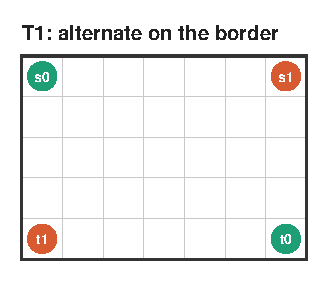
\includegraphics[height=2.6cm]{figures/cat_T1.pdf}\hfill
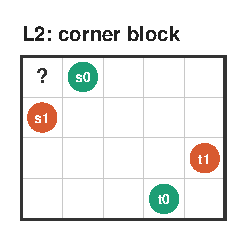
\includegraphics[height=2.6cm]{figures/cat_L2.pdf}\hfill
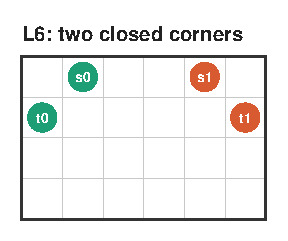
\includegraphics[height=2.6cm]{figures/cat_L6.pdf}\hfill
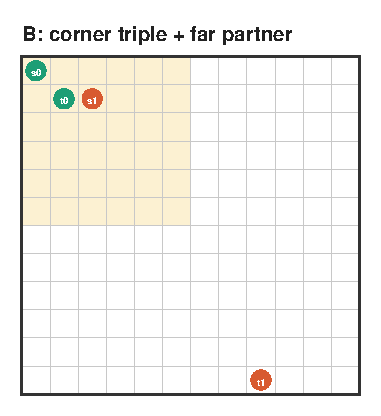
\includegraphics[height=3.6cm]{figures/cat_B.pdf}\hfill
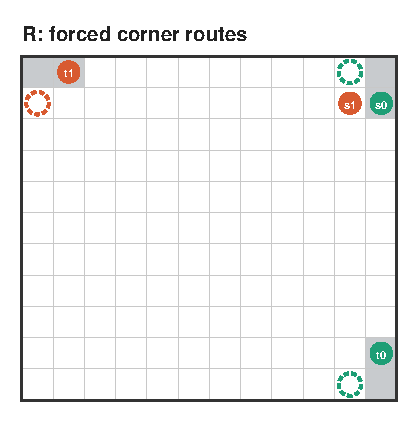
\includegraphics[height=3.6cm]{figures/cat_R.pdf}
\caption{Entries T1, L2, L6, B and R. In R, grey cells are settled by forced corner routes and
dashed circles mark the effective endpoints.}
\label{fig:catalogue}
\end{figure}

\paragraph{The R entry.}
Some corner patterns force a path through the corner cell. Rule R1: an endpoint at $(0,1)$ with
$(0,0)$ and $(1,0)$ empty forces its path through $(0,0)$ to $(1,0)$, so the endpoint effectively
sits at $(1,0)$ and the cells $(0,0), (0,1)$ are settled. Rules R2 (a same-colour diagonal at
$(0,0), (1,1)$) and R3 (a different-colour pair at $(1,2), (2,1)$) settle $2\times2$ and $3\times3$
corner regions similarly. After applying the rules in a fixed order, R fires if the effective
endpoints alternate along the border of the remaining region (T1 for that region).

\paragraph{Motivation for the entries.}
P and T1 are the classical obstructions: parity (each path alternates colours) and planarity (two
disjoint paths between alternating border points would cross). T2, L1--L6 and E1 express forced
degrees near endpoints and corners. B, C and D are the residue: corner configurations that are
unsolvable for reasons that are local but not short; each was found by exhaustive search on corner
windows, and each is certified by a window computation (Section~\ref{sec:proof}).

\section{The algorithm}\label{sec:algorithm}

\subsection{Reductions and band extension}

On an axis of length $n \ge 13$, the following reductions delete two free lines $d, d+1$:
\begin{itemize}
\item[(S)] \emph{strip}: an edge gap of at least $4$ lines (delete the outermost two);
\item[(K)] \emph{compression}: an internal gap of at least $10$ lines (delete two from its middle);
\item[(I)] \emph{interior compression}: an internal gap of at least $3$ lines containing $d, d+1$
  with $8 \le d \le n - 10$.
\end{itemize}

\begin{lemma}[Band extension]\label{lem:band}
If $I'$ is solvable and row $r$ of $I'$ is free, then inserting two empty rows directly below $r$
gives a solvable instance $I$. A solution of $I$ is obtained from one of $I'$ in time $O(RC)$.
\end{lemma}
\begin{proof}[Construction]
Stretch every path edge crossing below row $r$ through the two new rows. The new rows split into
blocks between consecutive crossings; each crossing absorbs the block on one of its sides by a
U-shaped detour. The remaining block is absorbed by a \emph{square flip}: a path edge
$(r, a)$--$(r, a{+}1)$ inside it is replaced by the block's boundary cycle. Such an edge exists by
counting: the $m$ crossing cells of row $r$ supply at most $m$ horizontal edges, while each of the
$m+1$ runs of non-crossing cells needs one (its cells have degree two and no vertical edge
downward).
\end{proof}

\begin{figure}[ht]
\centering
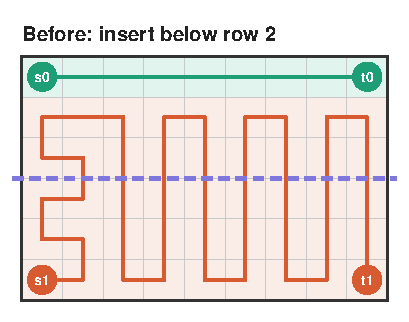
\includegraphics[height=3.2cm]{figures/band_before.pdf}\qquad
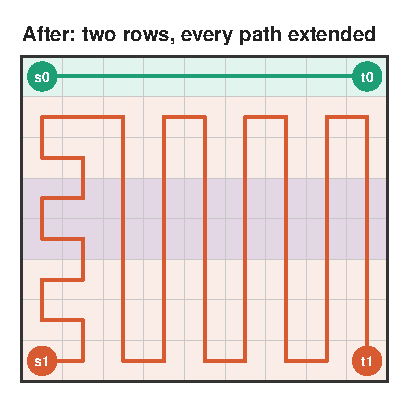
\includegraphics[height=3.8cm]{figures/band_after.pdf}
\caption{Band extension: two rows inserted below row 2.}
\label{fig:band}
\end{figure}

\subsection{Moves}

\begin{figure}[ht]
\centering
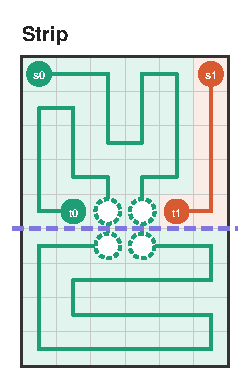
\includegraphics[height=4.3cm]{figures/move_strip.pdf}\hfill
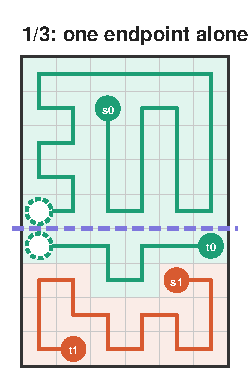
\includegraphics[height=4.3cm]{figures/move_13.pdf}\hfill
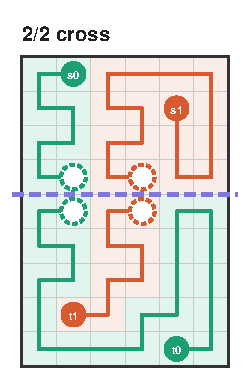
\includegraphics[height=4.3cm]{figures/move_cross.pdf}\hfill
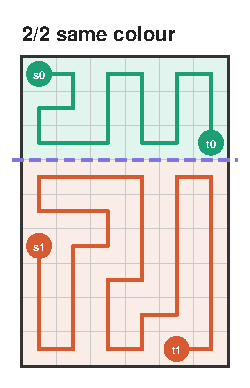
\includegraphics[height=4.3cm]{figures/move_same.pdf}\hfill
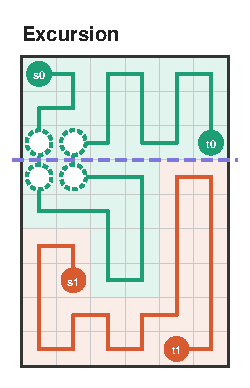
\includegraphics[height=4.3cm]{figures/move_exc.pdf}
\caption{The five move types: strip (an empty block is spliced in), 1/3, 2/2 cross, 2/2 same, and
excursion (colour \cA leaves its side and returns).}
\label{fig:moves}
\end{figure}

A move cuts the rectangle between rows $p-1$ and $p$ (up to symmetry). The types, by how the
endpoints fall (Figure~\ref{fig:moves}):
\emph{strip} (all endpoints on one side; the other side is empty, has even area and at least two
lines; its block is spliced into a path running along the cut);
\emph{1/3} (one endpoint alone; its piece is a one-path piece to its crossing);
\emph{2/2 cross} (one endpoint of each colour on each side; two crossings);
\emph{2/2 same} (each side holds one whole pair; two one-path pieces);
\emph{excursion} (each side holds one whole pair, and one colour crosses the cut twice).
Pieces' solutions glue along the crossing edges.

\subsection{Pseudocode}

Algorithm~\ref{alg:decide} decides an instance, Algorithm~\ref{alg:solve} constructs a solution, and
Algorithm~\ref{alg:band} is the band extension used to undo a reduction.

\begin{algorithm}[H]
\caption{Decision}\label{alg:decide}
\begin{algorithmic}[1]
\Require instance $I = (R, C, s_0, t_0, s_1, t_1)$ with four distinct endpoints
\Ensure whether $I$ is solvable
\If{$\min(R, C) \le 10$} \Return \Call{PlugDPFeasible}{$I$} \Comment{Appendix~\ref{app:plugdp}}
\Else\ \Return \textbf{not} \Call{Fires}{$I$} \Comment{Section~\ref{sec:catalogue}}
\EndIf
\end{algorithmic}
\end{algorithm}

\begin{algorithm}[H]
\caption{Construction}\label{alg:solve}
\begin{algorithmic}[1]
\Function{Solve}{$I$}
  \If{$\min(R, C) \le 10$} \Return \Call{PlugDPSolve}{$I$} \EndIf
  \If{\Call{Fires}{$I$}} \Return \textsc{None} \EndIf
  \If{$(\mathit{axis}, d) \gets$ \Call{FindReduction}{$I$} succeeds}
    \State $I' \gets I$ with lines $d, d+1$ on $\mathit{axis}$ deleted
    \State $S' \gets$ \Call{Solve}{$I'$}
    \State \Return \Call{BandExtend}{$S'$, $\mathit{axis}$, $d$} \Comment{Lemma~\ref{lem:band}}
  \EndIf
  \If{a cut separates the two pairs and both one-path pieces are acceptable}
    \State \Return the two Hamiltonian paths (IPS construction)
  \EndIf
  \State $M \gets$ \Call{FindMove}{$I$} \Comment{exists by Theorem~A; here $R, C \le 22$}
  \State solve each piece of $M$ (by IPS, the plug DP, or \Call{Solve}{})
  \State \Return the pieces' solutions glued along $M$'s crossings
\EndFunction
\Statex
\Function{FindReduction}{$I$}
  \For{$\mathit{axis} \in \{\text{rows}, \text{columns}\}$ with length $n \ge 13$}
    \If{lines $0..3$ are free} \Return $(\mathit{axis}, 0)$ \EndIf
    \If{lines $n{-}4..n{-}1$ are free} \Return $(\mathit{axis}, n-2)$ \EndIf
    \If{lines $\ell..\ell{+}9$ are free, with endpoints on both sides} \Return $(\mathit{axis}, \ell+4)$ \EndIf
    \If{$8 \le d \le n{-}10$, lines $d, d{+}1$ and $d{-}1$ or $d{+}2$ free, endpoints on both sides}
      \State \Return $(\mathit{axis}, d)$
    \EndIf
  \EndFor
  \State \Return \textsc{None}
\EndFunction
\Statex
\Function{FindMove}{$I$}
  \For{$m = 0, 1, \dots, 10$} \Comment{width of the widest thin piece; $0$: none}
    \For{each move type, each of the 8 orientations, each endpoint relabelling}
      \For{each cut position $p$ and crossing choice whose widest thin piece has width $m$}
        \If{every piece is OK (narrower piece checked first)} \Return the move \EndIf
      \EndFor
    \EndFor
  \EndFor
\EndFunction
\end{algorithmic}
\end{algorithm}

\begin{algorithm}[ht]
\caption{Band extension (Lemma~\ref{lem:band}), rows}\label{alg:band}
\begin{algorithmic}[1]
\Require a solution $P$ of $I'$; a free row $r$
\Ensure a solution of $I'$ with two empty rows $n_1 = r{+}1$, $n_2 = r{+}2$ inserted
\State shift every cell below row $r$ down by two
\State $X \gets$ columns $c$ where $P$ uses the edge $(r, c)$--$(r{+}3, c)$ \Comment{crossings}
\For{$c \in X$} replace the edge by $(r,c), (n_1,c), (n_2,c), (r{+}3,c)$ \EndFor
\State let $B_0, \dots, B_{|X|}$ be the column blocks of rows $n_1, n_2$ between crossings
\State $j \gets$ an index with $B_j = \emptyset$, or else one whose block contains a path edge
       $(r,a)$--$(r,a{+}1)$
\For{the $i$-th crossing $c$} absorb $B_{i-1}$ if $i \le j$, else $B_i$, by a U-detour replacing
     $(n_1,c)$--$(n_2,c)$ \EndFor
\If{$B_j \ne \emptyset$} replace $(r,a)$--$(r,a{+}1)$ by the boundary cycle of $B_j$ opened at
     $(n_1,a)$--$(n_1,a{+}1)$ \EndIf
\end{algorithmic}
\end{algorithm}

\subsection{Complexity}
Each reduction removes two lines, so at most $(R + C)/2$ reductions occur, each costing a catalogue
check ($O(R + C)$) and a band extension ($O(RC)$). Moves occur only on rectangles with both sides
at most $22$, in constant time. The total is $O((R + C)\,RC)$ for $R, C \ge 11$, plus the plug DP,
which is linear in the long side for a fixed short side.

\subsection{A worked example}

\begin{figure}[ht]
\centering
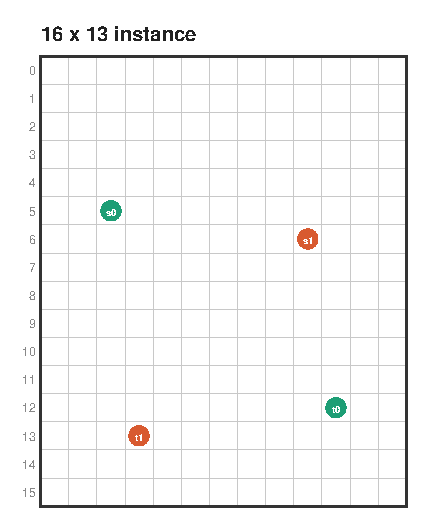
\includegraphics[height=4.4cm]{figures/ex_0.pdf}\hfill
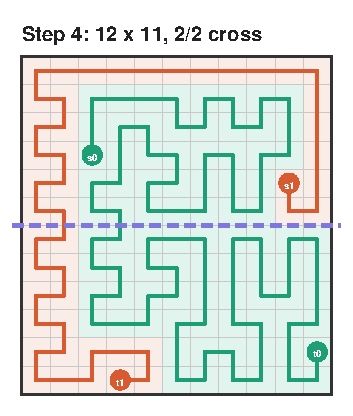
\includegraphics[height=4.0cm]{figures/ex_4.pdf}\hfill
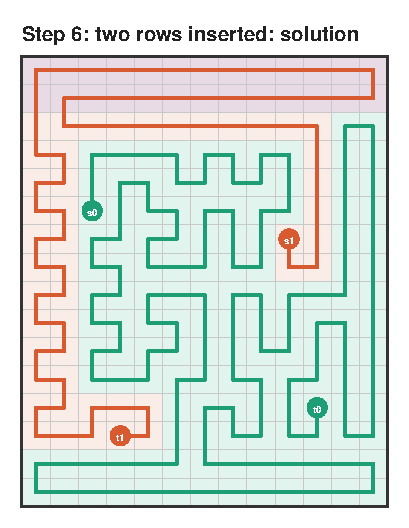
\includegraphics[height=4.4cm]{figures/ex_final.pdf}
\caption{A $16 \times 13$ instance; the $12\times11$ core with its 2/2-cross move; the solution.}
\label{fig:example}
\end{figure}

For the $16\times13$ instance of Figure~\ref{fig:example}: rows $0$--$3$ are free, so the strip
reduction deletes rows $0, 1$; the $14\times13$ result has no reduction, and strip moves cut off a
$2\times13$ block below and a $12\times2$ block on the right; the $12\times11$ core is split by a
horizontal 2/2-cross move into two thin $6\times11$ pieces, solved by the plug DP. The blocks are
spliced back and the two deleted rows reinserted by band extension.

\section{Proof outline}\label{sec:proof}

\begin{theorem}[Theorem B: soundness of the catalogue]
If an entry fires on an instance in $\Dom$, the instance is unsolvable.
\end{theorem}
P, T1, T2, L1--L6, E1 and R have direct proofs (parity; two disjoint paths between alternating
border points of a disc cross; forced degrees). B, C and D are certified by \emph{window
certificates}: a dynamic program over the corner window enumerates all ways a solution can look
inside it, and an outside test (parity, a non-crossing perfect matching of the boundary crossings,
path structure) shows that none can be completed outside, for any rectangle in $\Dom$.

\begin{theorem}[Theorem A: completeness of the catalogue]
Every instance in $\Dom$ that passes the catalogue is solvable.
\end{theorem}
By induction on the area. If a reduction applies, the smaller instance passes (each entry's view is
unchanged) and is solvable by induction; band extension lifts its solution. Otherwise both sides
are at most $22$ (a side $\ge 23$ always has a reduction); for these finitely many instances a valid
move exists (computer check), its thin pieces are solvable, its other two-path pieces are smaller
passing instances in $\Dom$, solvable by induction, and the pieces glue.

\section{Implementations}\label{sec:impl}

We provide libraries in Python (the reference), JavaScript and C, each with a command-line program.
All three implement Algorithms~\ref{alg:decide}--\ref{alg:band} and the plug DP with the same
iteration orders, and produce byte-identical output, including the paths. Testing:
\begin{itemize}
\item the catalogue of each implementation agrees with the Lean definition on $60{,}000$ random
  instances (sides $2$--$24$, endpoints clustered near corners);
\item the three implementations agree on $450$ random instances with sides $3$--$45$, and every
  reported solution is verified;
\item the C implementation solves $20{,}000$ random instances with sides $11$--$60$ in about
  $8$ seconds, with \textsc{Decide} and \textsc{Solve} agreeing on every instance;
\item on $300$ random instances with sides $11$--$12$, \textsc{Decide} agrees with an independent
  exact solver.
\end{itemize}

\section{Verification in Lean}\label{sec:lean}

The development is about $27{,}000$ lines of Lean~4~\cite{lean4} with Mathlib~\cite{mathlib20}.
The trusted statement is a short file defining instances, paths and solutions. The main results:
\begin{itemize}
\item \texttt{passes\_iff\_solvable}: for $R, C \ge 11$ and a well-formed instance,
  $\pass(I) \leftrightarrow \mathrm{Solvable}(I)$;
\item \texttt{thinBF\_iff}: the (proof-oriented) plug DP accepts iff the instance is solvable, for
  every rectangle, using only the standard axioms;
\item \texttt{solvableB\_iff}: a decision procedure for every rectangle is correct.
\end{itemize}
Here \pass is a computable Boolean function; the theorem is about it as defined, so no informal
transcription of the catalogue needs to be trusted. The IPS characterization is formalized as
well and used for one-path pieces.

\paragraph{Compromises.}
\begin{enumerate}
\item \emph{Computation by \nd.} The window certificates ($10$ theorems) and the base case
  ($144$ theorems, one per box of sides $11$--$22$) are evaluated by the Lean compiler rather than
  the kernel. This adds $154$ axioms that trust the compiler and the generated native code. Kernel
  evaluation is not practical: on a $6\times6$ window the kernel exceeded $16$\,GB after
  $20$~minutes on a computation the compiled code does in $3$~seconds, and an $8\times8$ window
  reaches $2.3\times10^5$ states.
\item \emph{Symmetry handling.} The base case checks one representative per orbit of the
  $64$-element symmetry group (geometric symmetries, colour swap, reversing either path). Instead
  of proving that the catalogue is invariant under reflections, the computation checks that the
  representative or one of its reflections passes; invariance under the other symmetries is proved.
  The search region is about $2.8\times10^{10}$ instances; the check takes about $16$ CPU-hours
  ($4$ hours on $4$ threads).
\item \emph{Checked search instead of verified search.} The move search is a Boolean function
  proved sound (a found move is valid); thin pieces are solved by an unverified solver and the
  solutions are checked by a verified checker.
\item \emph{Precompiled modules.} Without \texttt{precompileModules}, \nd interprets the
  project's functions and is about $400\times$ slower.
\item \emph{Running time.} The polynomial bound is not formalized; Lean has no standard cost model
  short of Turing machines. The theorems certify what is computed; the running-time analysis is
  on paper.
\item \emph{Thin case.} The verified plug DP uses a proof-friendly state encoding (sorted lists of
  pieces coded by their ends) rather than the bracket encoding of the implementations.
\end{enumerate}

\section{Discussion}

The characterization gives a linear-time decision procedure for two pairs on large rectangles, in
contrast with NP-completeness for unbounded $k$. Natural questions are three or more pairs on
rectangles, where corner interactions multiply, and two pairs on other regions such as solid grid
graphs. The catalogue's corner configurations (B, C, D) were found by computer; a conceptual
description of them would shorten the proof and might allow kernel-checked certificates.

\bibliographystyle{plain}
\bibliography{references}

\appendix

\section{The plug DP}\label{app:plugdp}

Transpose so that the grid has $W \le L$ rows. Cells are processed column by column, top to bottom.
The \emph{frontier} after some cells consists of $W + 1$ edges between processed and unprocessed
cells: one per row, plus the edge below the current cell (Figure~\ref{fig:frontier}). A state
assigns each frontier edge a 3-bit code: unused; an \emph{anchor} of colour \cA or \cB (a piece
ending at an endpoint); or an \emph{open} or \emph{close} bracket of colour \cA or \cB (a piece with
both ends on the frontier; matched like parentheses, since pieces cannot cross).

\begin{figure}[ht]
\centering
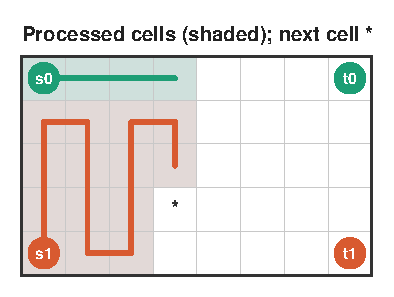
\includegraphics[height=3.2cm]{figures/plugdp_frontier.pdf}
\caption{Processed cells (shaded) and the next cell ($*$).}
\label{fig:frontier}
\end{figure}

\begin{algorithm}[ht]
\caption{Plug DP (decision)}\label{alg:plugdp}
\begin{algorithmic}[1]
\Function{PlugDPFeasible}{$I$} \Comment{$W \le L$ after transposition}
  \State $S \gets \{\text{all-empty}\}$
  \For{column $c = 0, \dots, L-1$}
    \If{$c > 0$} shift every state by one slot \EndIf
    \For{row $r = 0, \dots, W-1$}
      \State $S \gets \bigcup_{s \in S} \Call{Step}{s, r, c}$
    \EndFor
  \EndFor
  \State \Return all-empty $\in S$
\EndFunction
\Statex
\Function{Step}{$s, r, c$} \Comment{slot $r$: plug from above; $r{+}1$: from the left}
  \State $b \gets 1$ if $(r, c)$ is an endpoint of colour $k$, else $2$; $h \gets$ number of incoming plugs
  \If{$h > b$ or $b - h$ exceeds the free directions (right, down)} \Return $\emptyset$ \EndIf
  \If{$h = 0$}
    \State at an endpoint: a new anchor of colour $k$, going right or down
    \State otherwise: a new bracket pair of either colour, going right and down
  \ElsIf{$h = 1$}
    \State continue the plug right or down, or end it if $(r, c)$ is an endpoint of its colour
    \State (ending an anchor completes its path; ending a bracket makes its partner an anchor)
  \Else \Comment{join two plugs of the same colour}
    \State two anchors: path complete; an anchor and a bracket: the partner becomes an anchor
    \State close then open: the pieces merge; open then close: a cycle, rejected
    \State two opens or two closes: the outer partner's bracket type changes
  \EndIf
  \State \Return the resulting states (outgoing plugs in slots $r$ = right, $r{+}1$ = down)
\EndFunction
\end{algorithmic}
\end{algorithm}

\paragraph{Construction.} The forward pass stores one checkpoint (the state set) per column. A
backward pass re-runs each column from its checkpoint, recording predecessors and keeping only
states whose processed slots agree with the known end-of-column state, then traces back the chosen
edges. The number of states is bounded by the number of valid frontiers (about $10^5$ for
$W = 10$), so the running time is $O(L \cdot W \cdot \#\text{states})$.

\paragraph{Correctness.} By induction over the cells, the reachable states are exactly the
signatures (used frontier edges, their pairing, and the colours of pieces ending at endpoints) of
partial solutions on the processed cells; hence the empty final state is reachable iff a solution
exists. Lean verifies this for an equivalent DP with a different encoding.

\section{The listed corner configurations}\label{app:lists}

Cells are written $ij$ for frame coordinates $(i, j)$.

\noindent\textbf{B} ($RC$ even; triples $(p\,q\,r)$: colour $a$ at $p, q$, $\bar a$ at $r$):
(00 11 12), (01 02 11), (01 02 12), (01 03 11), (01 04 11), (01 04 12), (01 05 11), (01 12 11),
(01 12 13), (01 12 22), (01 12 31), (01 13 03), (01 21 13), (01 21 22), (01 21 31), (02 21 10),
(03 11 10), (04 11 10), (04 21 10), (04 21 12), (05 11 10).

\noindent\textbf{B} ($R$, $C$ odd): (00 11 12), (00 11 22), (01 02 11), (01 04 11), (04 11 10).

\noindent\textbf{C} ($RC$ even; $\{$one pair $\mid$ the other pair$\}$):
\{01 03 $\mid$ 11 13\}, \{01 06 $\mid$ 07 11\}, \{01 06 $\mid$ 11 70\}, \{01 06 $\mid$ 12 60\},
\{01 07 $\mid$ 11 60\}, \{01 13 $\mid$ 11 12\}, \{01 13 $\mid$ 12 22\}, \{01 13 $\mid$ 12 31\},
\{01 22 $\mid$ 11 12\}, \{01 22 $\mid$ 12 31\}, \{01 22 $\mid$ 13 30\}, \{01 70 $\mid$ 11 60\},
\{02 11 $\mid$ 21 30\}, \{02 20 $\mid$ 12 21\}, \{03 21 $\mid$ 31 40\}, \{06 21 $\mid$ 12 60\},
\{12 22 $\mid$ 13 21\}, \{12 31 $\mid$ 13 21\}, \{01 12 $\mid$ 04 22\}, \{01 12 $\mid$ 04 31\},
\{01 12 $\mid$ 13 20\}, \{01 12 $\mid$ 13 40\}, \{01 12 $\mid$ 20 22\}, \{01 12 $\mid$ 22 40\},
\{01 12 $\mid$ 31 40\}, \{01 13 $\mid$ 03 04\}, \{01 13 $\mid$ 03 20\}, \{01 13 $\mid$ 03 40\},
\{01 21 $\mid$ 02 22\}, \{01 21 $\mid$ 02 31\}, \{01 21 $\mid$ 04 13\}, \{01 21 $\mid$ 04 22\},
\{01 21 $\mid$ 04 31\}, \{01 21 $\mid$ 13 40\}, \{01 21 $\mid$ 22 40\}, \{01 21 $\mid$ 31 40\}.

\noindent\textbf{D} ($RC$ odd): \{00 01 $\mid$ 11 20\}, \{00 14 $\mid$ 02 13\}, \{00 23 $\mid$ 02 13\}.

\end{document}
